% ---------------------------------------------------
% ------- Praktikum Versuchsprotokoll ---------------
% ---------------------------------------------------
% Erstellt: 	2022, Dustin Brunner
% Lizenz: 		Creative Commons Namensnennung 4.0 International (CC BY 4.0)
% ---------------------------------------------------

% ------ Variaben für jeweiligen Versuch anpassen ---
\def\Versuchsname{<Versuchsname>}
\def\Modulname{<Modulname>}
\def\Versuchsdatum{<Versuchsdatum>}
\def\Abgabedatum{<Abgabedatum>}

% ---------------------------------------------------
% ------- Dokument Konfigurieren --------------------
% ---------------------------------------------------
\documentclass[
paper=a4,			% A4 Papier
german,				% Dokumentensprache Deutsch
parskip=half,		% Europäischer Satz mit Abstand zwischen Absätze
twoside=false,		% Papier einseitig bedruckt (auch für Onlineanwendungen)
fontsize=12pt,		% Schriftgröße
%headsepline,        % Linie nach Kopfzeile
%footsepline,        % Linie vor Fusszeile
]{scrartcl}

% ---------------------------------------------------
% ------- Pakete ------------------------------------
% ---------------------------------------------------

% --- Allgemeine Pakekte für Dokumentenkonfiguration ---
\usepackage[utf8]{inputenc}  	% Codierung der Datei
\usepackage[T1]{fontenc}  		% Vollen Umfang der Schriftzeichen + Sonderzeichen
\usepackage[ngerman]{babel}  	% Sprache auf Deutsch (neue Rechtschreibung)

\usepackage{graphicx} 			% Bilder einbinden 
								% \begin{figure}[H]
								%	\centering
								%	\includegraphics[scale=0.6]{Pfad/zur/Datei}
								%	\caption{Bildunterschrift}
								%	\label{fig:Versuchsaufbau} % Kurzname für Verweise im Text: Abbildung~\ref{fig:Versuchsaufbau}
								% \end{figure}
\usepackage{float}				% Option "H" für Bilder: Bilder an Fester Position im Text
								
\usepackage{caption} 			% Bildunterschriften, TabellenÜBERschriften
%\usepackage{subcaption}  		% Unterabbildungen, Untertabellen (meherere Abblidungen pro Zeile)

% --- Mathematik, Formeln und Einheiten -----------
\usepackage{amsmath}			% Mathe-Umgebung
\usepackage{amssymb}			% Zusatzsymbole für Formeln
\usepackage[					% SI-Einheiten, Beispiele:
								% Wert + Unsicherheit + Einheit: $\SI{4,15+-0,01}{\meter \per \second}$ 
								% Wert + Einheit:				 $\SI{4,15}{\meter \per \second}$
								% nur Einheit: 					 $\si{\meter \per \second}$
locale=DE,
separate-uncertainty,  			% Unsicherheiten mit ± angeben
]{siunitx}
\usepackage{physics}  			% Erstellung von Gleichungen vereinfachen
								% (http://mirrors.ibiblio.org/CTAN/macros/latex/contrib/physics/physics.pdf)
\usepackage{array}				% Mehrzeilige Formeln am "&"-Symbol ausrichten (für = z.B. &=&)
\usepackage{cancel}				% Kürzen/Durchstreichen mit \cancel, \bcancel und \xcancel


% --- Gestaltung ----------------------------------
%\usepackage{microtype}  		% Mikrotypographie (kann man am Ende verwenden)
\usepackage{lmodern} 			% Schriftart (z.B. lmodern oder mathptmx = Times)
%\usepackage[toc]{multitoc}  	% mehrspaltiges Inhaltsverzeichnis
\usepackage{csquotes}  			% Anführungszeichen mit \enquote
\setlength{\parindent}{0em} 	% Einzüge bei neuem Absatz verhindern

%\usepackage{enumitem}  		% Abstände zwischen Listenpunkten verringern (beide Zeilen auskommentieren)
%\setlist{itemsep=-10pt}

\usepackage[table]{xcolor}		% Farbige Schrift, auch in Tabellen (z.B. {\color{red}Testtext})

%\usepackage{multirow}			% Zellen vertikal verbinden z.B. \multirow[t,c,b]{#Zeilen}{Breite der Spalte}{Inhalt}
\newcolumntype{C}[1]{>{\centering\arraybackslash}p{#1}} %Zentrierte Spalte fester Breite z.B. C{2cm} 
\usepackage[hidelinks]{hyperref}% Links, Metadaten und weitere PDF-Features

								% PDF-Metadaten setzen
\hypersetup{pdfauthor={<PDF-Autor hier eintragen>}, pdftitle={\Modulname, \Versuchsname}}  	

\usepackage{pdfpages}
% --- Kopf- und Fußzeilen -------------------------
\usepackage[
automark,
headsepline,					% Linie unter Kopfzeile
]{scrlayer-scrpage}
\clearpairofpagestyles			% Aktuelle Kopf- und Fußzeilen Konfiguration löschen
								% Texte für Kopf- und Fußzeilen
\ihead{Praktikum \Modulname \\\Versuchsname}		
\ohead{<PDF-Autor hier eintragen>, Partner 1\\ Partner 2}

\usepackage{lastpage}			% Seitenzahl der letzten Seite (für Fußzeile)
\cfoot{Seite \thepage \ von \pageref{LastPage}}

% Alternative Kopf- und Fußzeilen Konfiguration, nicht empfohlen in Verbindung mit scrartcl
%\usepackage{fancyhdr}
%\pagestyle{fancy}
%\fancyhf{}
%\rhead{<PDF-Autor hier eintragen>}
%\lhead{Praktikum <Modulname>}
%\usepackage{lastpage}
%\cfoot{Seite \thepage \ von \pageref{LastPage}}


% --- Manipulation des Seitenstils ----------------
%\addtolength{\oddsidemargin}{-1in}		% Seitenränder in cm setzten
%\addtolength{\textwidth}{1in}
%\addtolength{\oddsidemargin}{2cm}
%\addtolength{\textwidth}{-2cm}
%\addtolength{\topmargin}{-1in}
%\addtolength{\topmargin}{2cm}
%\addtolength{\textheight}{1in}

\newcommand{\paragraphlf}[1]{\paragraph{#1}\mbox{}\\} % Neue Zeile nach Paragraphtitel


\begin{document}
	
\begin{titlepage}				% Titelseite
	%\vspace*{1cm}
	\begin{center}
		\begin{LARGE}
			{\fontfamily{cmr}\textsc{\textbf{Universität Musterstadt}}}\\
			Fakultät für XYZ\\
			Professur für ABC\\
		\end{LARGE}
		\hrulefill
		
		\vspace{1cm}
		{\LARGE Praktikum}\\
		{\huge \textbf{\Modulname{}}}\\
		\vspace{1cm}
		{\LARGE Versuch:}\\
		{\huge \textbf{\Versuchsname{}}}\\
	
		\vspace{1cm}
	\end{center}

	\begin{large}
		\begin{tabbing}
			Versuchsdatum: 	\quad\= \Versuchsdatum{} \quad\quad\= Abgabedatum: \quad \Abgabedatum{}\\\\
			
			Laborgruppe: 	\> <Gruppenname>\\\\
			
			Mitarbeiter:	\> <PDF-Autor hier eintragen>\\
							\> Partner 1\\
							\> Partner 2\\\\
			Email:			\> \href{mailto:mail@example.com}{<mail@example.com>}\\\\
			
			Betreuer:		\> <Betreuer Name> \\
		\end{tabbing}
	\end{large}
	
	\hrulefill
\end{titlepage}	


\section{Aufgabenstellung}
	Lorem ipsum dolor sit amet, consectetur adipisici elit, sed eiusmod tempor incidunt ut labore et dolore magna aliqua. Ut enim ad minim veniam, quis nostrud exercitation ullamco laboris nisi ut aliquid ex ea commodi consequat. Quis aute iure reprehenderit in voluptate velit esse cillum dolore eu fugiat nulla pariatur. Excepteur sint obcaecat cupiditat non proident, sunt in culpa qui officia deserunt mollit anim id est laborum. 
			
%------------------------------------------------------------------------------------------------

\section{Grundlagen}
	Lorem ipsum dolor sit amet, consectetur adipisici elit, sed eiusmod tempor incidunt ut labore et dolore magna aliqua.

\subsection{Bilder}

	\begin{figure}[H]
		\centering
		
\includegraphics[scale=0.2]{pictures/platzhalter_bild.png}
		\caption{Bild einzeln zentriert}
		\label{fig:platzhalter_bild}
	\end{figure}

	Im Text kann auf Abbildung~\ref{fig:platzhalter_bild} verwiesen werden.
	
	\newpage 
	
	Zwei Abbildungen nebeneinander:
	
	\begin{figure}[H]
		\centering
		\begin{minipage}{0.45\linewidth}
			
\includegraphics[width=1.0\linewidth]{pictures/platzhalter_bild.png}
			\caption{Linkes Bild}
			\centering
			\label{fig:platzhalter_bild2}
		\end{minipage}\hspace{2em}%\hfill%
		\begin{minipage}{0.45\linewidth}
			
\includegraphics[width=1.0\linewidth]{pictures/platzhalter_bild.png}
			\caption{Rechtes Bild}
			\centering
			\label{fig:platzhalter_bild3}
		\end{minipage}
	\end{figure}
	

\subsection{Gleichungen}
	Eine Gleichung mit Erläuterungen zu den Verwendeten Variablen. 
	\begin{equation}
		\label{eq:Ohmsches_Gesetz}
		R = \frac{U}{I}
	\end{equation}
	\begin{tabular}[H]{lcp{12cm}}
		$R$ & $-$ & Widerstand in $\si{\ohm}$ \\
		$U$ & $-$ & Spannung in $\si{\volt}$ \\
		$I$ & $-$ & Stromstärke in $\si{\ampere}$ \\
	\end{tabular}

	Im Text kann auf Gleichung~\ref{eq:Ohmsches_Gesetz} verwiesen werden.
	
	
	Eine Gleichung ohne Erläuterungen:
	\begin{equation}
		\label{eq:Normalverteilung}
		h(x) = \frac{1}{\sigma \sqrt{2\pi}}\cdot e^{-\frac{(x-\mu)^2}{2\sigma^2}}
	\end{equation}

	Gleichungsumgebung für ausführliche Berechnungen:
	\begin{equation*}
		\begin{split}
			R &= \frac{U}{I} \\
			  &= \frac{\SI{100}{\milli \volt}}{\SI{5}{\ampere}} \\
			  &= \frac{100 \cdot 10^{-3} \si{\volt}}{\SI{5}{\ampere}} \\
			R &= \SI{0,02}{\ohm} = \underline{\underline{\SI{20}{\milli \ohm}}}.
		\end{split}
	\end{equation*}

\subsection{Tabellen}
Eine Beispiel-Tabelle für Messwerte:
\begin{table}[H]
	\centering
	\caption{Messwerte}
	\label{tab:Messwerte}
	\setlength{\extrarowheight}{3pt}
	\begin{tabular}{C{1.8cm}|C{1.8cm}|C{1.8cm}}
		\rowcolor[gray]{.9}
		$U \:/\: \si{\volt}$	& $U_{2} \:/\:\si{\milli \volt}$	& $I \:/\:\si{\nano \ampere}$ \\
		\hline\hline
		1,2						& 3,4			& 5,67 \\
		\hline
		8,910					& 11,12			& 13,14 \\
		\hline
		1,2						& 3,4			& 5,67 \\
		\hline
		8,910					& 11,12			& 13,14 \\
		
	\end{tabular}
\end{table}

\subsection{Weitere nützliche Befehle}
	Texte in \enquote{Anführungszeichen} mit \verb|\enquote{}|
	
	Quelltext-Formatierung s.o.
	
	Inline-Formel: Der Wert des Widerstandes beträgt: $R = \SI{100}{\ohm}$.
	
	Einheiten ohne Zahlenwert $\si{\ohm}$ und mit Zahlenwert $\SI{100}{\ohm}$.
	
	Zitat einer Quelle: \cite{Versuchsanleitung}.
	
\subsection*{Unnummerierte Abschnitte, Formeln, etc. mit \enquote{*}}
	
	
%------------------------------------------------------------------------------------------------

\section{Versuchsaufbau}
	 Lorem ipsum dolor sit amet, consectetur adipisici elit, sed eiusmod tempor incidunt ut labore et dolore magna aliqua.

%------------------------------------------------------------------------------------------------	

\section{Durchführung und Auswertung}
	Lorem ipsum dolor sit amet, consectetur adipisici elit, sed eiusmod tempor incidunt ut labore et dolore magna aliqua. Ut enim ad minim veniam, quis nostrud exercitation ullamco laboris nisi ut aliquid ex ea commodi consequat. Quis aute iure reprehenderit in voluptate velit esse cillum dolore eu fugiat nulla pariatur. Excepteur sint obcaecat cupiditat non proident, sunt in culpa qui officia deserunt mollit anim id est laborum. 



%------------------------------------------------------------------------------------------------

\section{Ergebnisse und Diskussion}
	Lorem ipsum dolor sit amet, consectetur adipisici elit, sed eiusmod tempor incidunt ut labore et dolore magna aliqua. Ut enim ad minim veniam, quis nostrud exercitation ullamco laboris nisi ut aliquid ex ea commodi consequat. Quis aute iure reprehenderit in voluptate velit esse cillum dolore eu fugiat nulla pariatur. Excepteur sint obcaecat cupiditat non proident, sunt in culpa qui officia deserunt mollit anim id est laborum. 
	
%------------------------------------------------------------------------------------------------

%Literaturverzeichnis
\begin{thebibliography}{}
	\bibitem{Versuchsanleitung}
	Professur XYZ:	\emph{Versuchsanleitung zum Versuch <Versuchsname>}
	
	\bibitem{samplepdf}
	africau.edu:
	\emph{A Simple PDF File}, \url{http://www.africau.edu/images/default/sample.pdf}, 20.\,Mar.~2022.
\end{thebibliography}



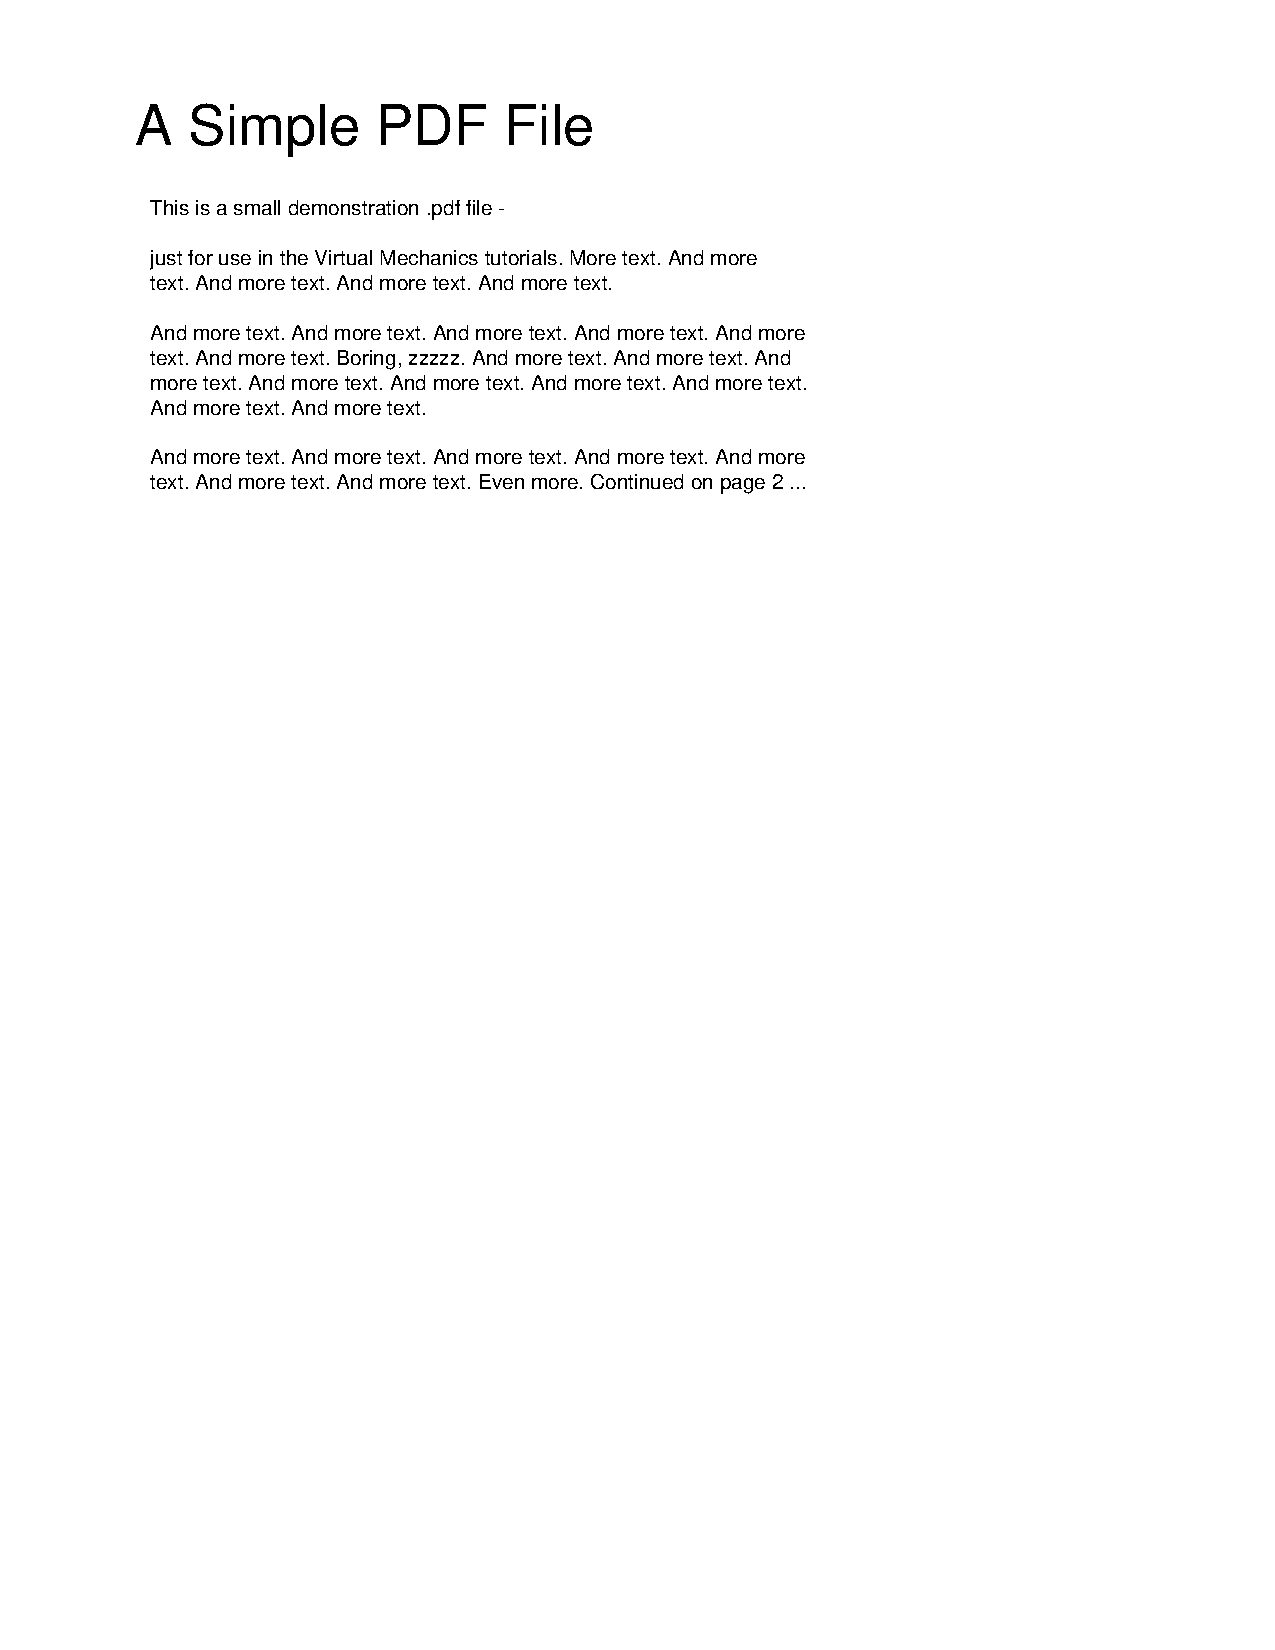
\includepdf[pages=1-2]{sample_attachment.pdf}
\end{document}